\section{Discussion of model}
In this section we will make an analysis of the different parts and 
parameters of the model and see what their role in the model is as well 
as inspect their domains and limitations. 

\subsection{The time steps}
In this section discuss how to set the the time steps of the calculation. 
When we do the simulations we want it be as cheap as possible. That is we want it to be done with as few calculations a possible. Because the cheaper you make the simulations the more pedestrians you can have in your simulation without waiting to long for the results to come out. One of the way to minimize the number of calculations is by choosing the highest possible value for $\Delta t$. For instant there would be no reason to make a simulation in a time step making people move so little that they, in the same time step in real life, would not be able to make a reaction on the changes.  
On the other hand there will of course be a maximum we can choose if we still want the simulations to look realistic. If all the pedestrians make big jumps in each time step it will not be very good to compare with real life situations. So we have to make sure that people are not able to land on top of each other or to pass through a wall because the repulsion forces are calculated at to great a distance compared to how big jumps a pedestrian can make.
So one of the big challenges when doing simulations is to choose the right value for $\Delta t$. One way to get a quantitative value for $\Delta t$ is by looking at at the size of the parameters added to the model to get some idea about the maximum displacement of a pedestrian as a function of time and then choose a value that seems reasonable.

\subsubsection{Linear approximation}
In our simulation, we use Euler's method to approximate solutions to the equations of motion, which are ordinary differential equations with initial conditions calculated from last time step, and those initial value problems look like:

\begin{eqnarray}
\frac{dy}{dt} &=& f(y),\\
y(t_{0}) &=& y_{0}
\end{eqnarray}

Within some small time interval from $t_{0}$ to $t_{0}+\bigtriangleup t$, the function of $ y(t) $ can be approximately represented by a straight line:

\begin{equation}
l(t) = y_{0} + f(y_{0}) (t-t_{0})
\end{equation}

then after a small step size, the function value $ y $ becomes
\begin{equation}
y = y_{0} + f(y_{0}) \bigtriangleup t
\end{equation}
and the calculated value of $ y $ also becomes the initial value for the following step. However, this kind of method can cause error in most situations, and there are methods trying to minimize the error caused by the numerical way of solving problem.

\subsubsection{Step size}
We can see that the error caused by the numerical approach must depends on the step size.  From the mathematical point of view, a smaller step size generally gives smaller error, but as we use the computer to do the calculation and it only deals with rational numbers, so the round off error becomes prominent. Therefore, an optimal step size could be the one that causes the sum of two sources of errors smallest.



\subsection{The fluctuation term}
In addition to all the forces action on the agent the change in velocity of agent 
$\alpha$ is controlled by fluctuation term. The role and nature of this term will 
be discussed in this subsection.

For the acceleration of pedestrian $\alpha$ we have following equation to add up the forces

\begin{equation}
\frac{d\vec{v}_{\alpha}}{dt}=\vec{f}_{\alpha}(t)+\vec{\xi}_{\alpha}(t)
\end{equation}

In this equation, $\vec{f}_{\alpha}(t)$ is the forces acting on pedestrian $\alpha$. The term $\vec{\xi}_{\alpha}(t)$
is called a fluctuation term and is added to the equation to reflect random behaviour of a pedestrian, in this case $\alpha$. In other words, $\vec{\xi}$ adds a stochastic behaviour to the model for each person and because of this, one can't expect the same simulation to give the completely same result as a previous simulation with the same initial conditions. The reason this term is added is that you would'nt expect every person to act with optimal behaviour in all situations. In some way you could also say that $\xi$ is a personality factor, taking into account the little differences in the behaviour of different persons.

When we choose a value for $\xi$ for each pedestrians, it is of course important that the pedestrians in the model will still behave in a way that are realistic. Therefore we do not want the fluctuation term to be the dominant factor that makes a person jump 5 meter for no reason. Instead it should be the little difference that in some cases makes a pedestrian, $\alpha$, go left instead of going right when passing another pedestrian, $\beta$, or something similar.  

When a reasonable mean value for $\xi$ have been chosen a good way to make a value for each pedestrian would be with the Gaussian distribution function. This would make the main part of the pedestrians have almost the same value but of certain percentage of the pedestrians would have greater or lower value representing different personalities like old people or children, or people in panic or people that in some other ways have disabilities. 


\subsection{The impatience/nervousness factor}
The impatience or nervousness factor is active when one calculates the force action 
on agent $\alpha$ from the velocity of the agent. This means that the agents earlier 
velocity alone will take a part in deciding the future velocity of the agent. This 
force is controlled by the impatience or nervousness factor. The impatience or 
nervousness factor is as stated earlier given by:

\begin{equation}\label{n}
    \eta_{\alpha} \left( t \right) =
    1 - \frac{\overline{V}_{\alpha} \left( t \right)}
             {V_{\alpha}^{0} \left( 0 \right)}
\end{equation}

where $\overline{V}$ is the average speed in the desired direction and as 
earlier $V_{\alpha}^{0} \left( 0 \right)$ is the speed at the beginning of the 
first calculation step of the simulation.

The impatience or nervousness factor i directly seen in the expression for 
$V_{\alpha}^{0}$.

\begin{equation}\label{v0}
    V_{\alpha}^{0}(t) = \left[ 1 - \eta_{\alpha} \left( t \right) \right] 
    V_{\alpha}^{0} \left( 0 \right) +
    \eta_{\alpha} \left( t \right)V_{\alpha}^{\text{max}}
\end{equation}

In the case where $0 \leq \eta_{\alpha} \leq 1$ the expression for 
$V_{\alpha}^{0} \left( t \right)$  makes sense. Here we can see why this term 
is called the impatience of the agent. If the fraction  between the average 
speed in the desired direction and the initial speed is low then $\eta_{\alpha} \approx 1$. 
When the impatience term is close to one $V_{\alpha}^{0} \left( t \right)$ 
is dominated by $V_{\alpha}^{\text{max}}$. That is, if the agent have not 
moved very far in the desired direction compared to the initial speed the 
impatience of the agent will cause the agent's future velocity to be dominated by 
the desired velocity of the agent.

If the agent has been moving in the desired direction with his initial 
speed the entire time then $\eta_{\alpha} = 0$  and 
$V_{\alpha}^{0} \left( t \right)$ will continue to be $V_{\alpha}^{0} \left( 0 \right)$.

In the case where $\eta_{\alpha} \leq 0$ that is the agent has moved further 
in the desired direction then he would have had he been walking with his 
initial speed. The expression for $V_{\alpha}^{0} \left( t \right)$
stats yield strange results. That $\eta_{\alpha} \leq 0$ would imply that:

\begin{equation}
    V_{\alpha}^{0} = \left[ 1 + \eta_{\alpha} \left( t \right) \right] 
    V_{\alpha}^{0} \left( 0 \right) -
    \eta_{\alpha} \left( t \right)V_{\alpha}^{\text{max}}
\end{equation}

And this will yield a negative value for $V_{\alpha}^{0}$ if $\left[ 1 + \eta_{\alpha} \left( t \right) \right] 
V_{\alpha}^{0} \left( 0 \right) < \eta_{\alpha} \left( t \right)V_{\alpha}^{\text{max}}$. 
This is a problem because it is not that far fetched that an agent will be 
forced to exceed his desired velocity.

In the case where $1 \leq \eta_{\alpha}$ it would mean that the agent has moved 
further in the opposite direction than the desired one and this can only happen very 
weird situations.\\

Equation (\ref{n}) and Equation (\ref{v0}) contains an intermediate variable $ n_{\alpha} \left( t \right) $, so in principle we are allowed to eliminate $ n_{\alpha} \left( t \right) $ and only show the relationship between $ V_{\alpha}^{0}(t) $ and $ \overline{V}_{\alpha} \left( t \right) $.  Thus we get

\begin{equation}\label{vv}
    V_{\alpha}^{0}(t) = \left[ 1 - \frac{v_{\alpha}^{max}}{v_{\alpha}^{0}(0)}\right]\overline{V}_{\alpha} \left( t \right) + v_{\alpha}^{max}
\end{equation}

Figure (\ref{impatience}) is a drawing of the graph about those two variables, and the intersection of the function line with both axis are $ (0, v_{\alpha}^{max}) $ and $ (v_{\alpha}^{max}\frac{v_{\alpha}^{0}(0)}{v_{\alpha}^{max}-v_{\alpha}^{0}(0)}, 0) $. Now there is a doubt whether the value of $ \overline{V}_{\alpha} \left( t \right) $ can reach $ v_{\alpha}^{max}\frac{v_{\alpha}^{0}(0)}{v_{\alpha}^{max}-v_{\alpha}^{0}(0)} $, if we have already set $ v_{\alpha}^{max} $ a fixed number for a certain agent.\\\\

In the case 
\begin{equation}
 v_{\alpha}^{max} \geq v_{\alpha}^{max}\frac{v_{\alpha}^{0}(0)}{v_{\alpha}^{max}-v_{\alpha}^{0}(0)}
\end{equation}

we get the relation
\begin{equation}
v_{\alpha}^{0}(0)\leq \frac{1}{�2}v_{\alpha}^{max}
\end{equation}

\begin{figure}
\centering
{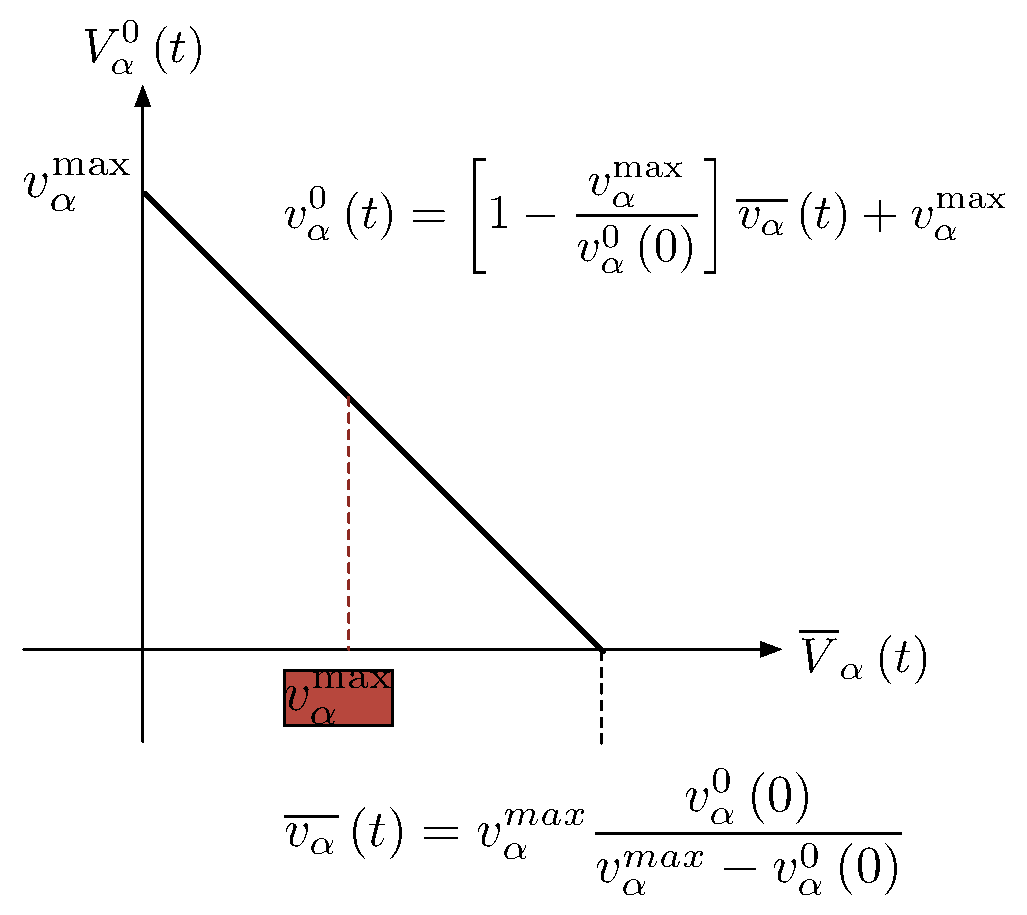
\includegraphics[scale=0.45]{impatience.pdf}} 
\caption{\small{The function about the desired velocity $ V_{\alpha}^{0}(t) $ 
and the average velocity in the desired direction of motion $ \overline{V}_{\alpha} \left( t \right) $}}
\label{impatience}
\end{figure}


\subsection{The repulsive interaction force}
From the given formula for calculating the repulsive force between agents in 
the description of the model, the part calculating the force to keep the 
personal space can be omitted when the agents are rather close to each other, 
then the calculation can be reduced as Equation (%\ref{re}).

\begin{equation}\label{re}
\overrightarrow{f_{\alpha\beta}}(t) = A_{\alpha}^{2} exp\left[ \frac{r_{\alpha\beta} - d_{\alpha}\beta}{B_{\alpha}^{2}}\right]  \overrightarrow{n_{\alpha\beta}}
\end{equation}

Taking the norms of both sides of Equation (\ref{re}), we can draw the 
relation between the value of $$ \overrightarrow{f_{\alpha\beta}}(t) $$ and $ d_{\alpha\beta} $, as in Figure (\ref{physicalinteraction}).\\

\begin{figure}
    \centering
    {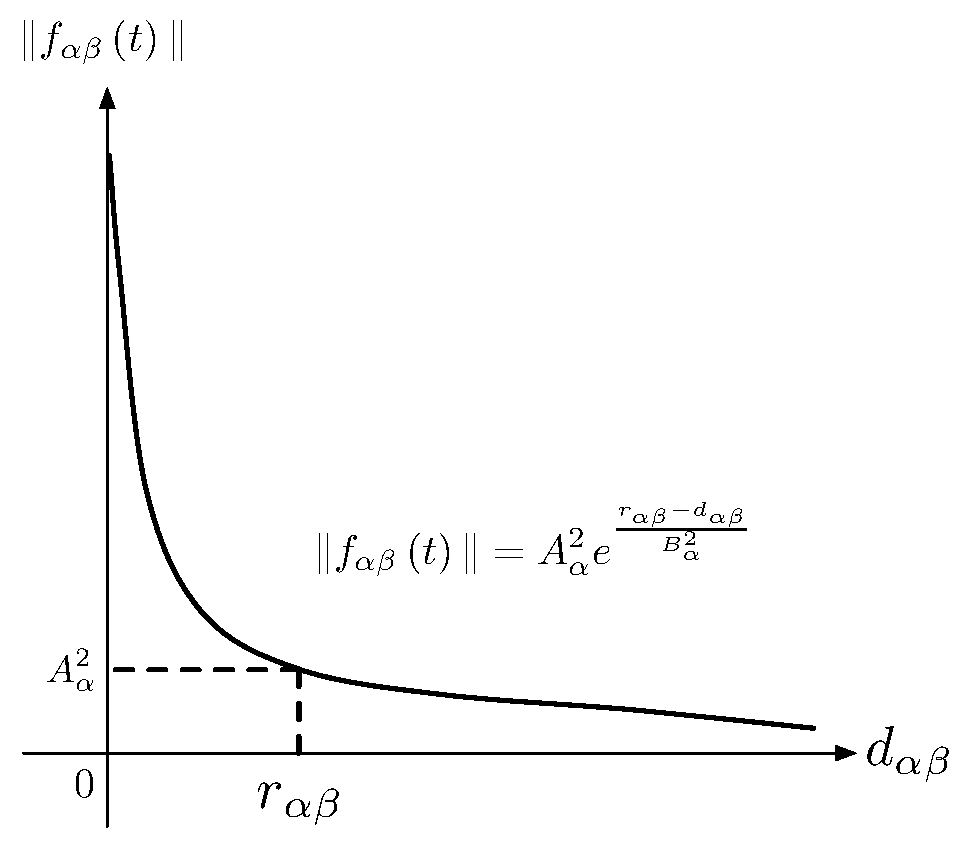
\includegraphics[scale=0.45]{physicalinteraction.pdf}} 
    \caption{The function about the interaction force 
        $f_{\alpha\beta}(t)$ and the distance between two agents
        $d_{\alpha \beta}$ }
    \label{physicalinteraction}
\end{figure}

There is one intersection of the graph and the axis $ \left( 0, A_{\alpha}^{2} exp\left( \frac{r_{\alpha\beta} }{B_{\alpha}^{2}}\right)  \right)  $. If put into the constants, we will be able to get a maximum value of $ f_{\alpha\beta}(t) $, since the distance between agents cannot be negative. Here we set $ A_{\alpha}^{2} = 3 m/s^{2} $, $ r_{\alpha\beta} = 0.6 m $, and $ B_{\alpha}^{2} = 0.2 m $, so $ f_{\alpha\beta}(t)^{max} \doteq 60 m/s^{2} $, which is about six times the gravitational acceleration and represents a rather large force between agents (as large as six person's weight). \\\\
However, we notice that the effective part of the force calculated above is only the horizontal component that enables the agent to move horizontally in the plane where we do the simulation, but the reality is that the agents sometimes are also able to move vertically, for example, by stepping upon other people when they cannot take the pushing force from the surrounding agents. When that happens, the horizontal component of the repulsive force becomes smaller even if $ d_{\alpha\beta} $ is kept the same(may need a graph to illustrate that)\\

Therefore, a qualitative modification of dependence between $ f_{\alpha\beta}(t) $ and $ d_{\alpha\beta} $ could be:\\
(add another drawing)

